\documentclass[10pt]{article}
\usepackage[polish]{babel}
\usepackage[utf8]{inputenc}
\usepackage[T1]{fontenc}
\usepackage{amsmath}
\usepackage{amsfonts}
\usepackage{amssymb}
\usepackage[version=4]{mhchem}
\usepackage{stmaryrd}
\usepackage{graphicx}
\usepackage[export]{adjustbox}
\graphicspath{ {./images/} }

\title{LIGA MATEMATYCZNA STYCZEŃ 2011 SZKOŁA PONADGIMNAZJALNA }

\author{}
\date{}


\begin{document}
\maketitle
\section*{ZADANIE 1.}
Wewnątrz trójkąta równobocznego \(A B C\) wybrano dowolny punkt \(P\). Punkty \(D, E, F\) są rzutami prostokątnymi punktu \(P\) na boki odpowiednio \(A B, B C, C A\). Wyznacz wartości, jakie może przyjmować wyrażenie

\[
\frac{P D+P E+P F}{A D+B E+C F}
\]

\section*{ZADANIE 2.}
Wyznacz wszystkie trójki \((a, b, c)\) liczb całkowitych, dla których \(a^{2}-b^{2}-c^{2}=1 \mathrm{i} a-b-c=-3\).

\section*{ZADANIE 3.}
W polach tablicy \(4 \times 4\) umieszczono liczbę -1 oraz piętnaście liczb 1. Można jednocześnie zmienić znaki wszystkich liczb w jednym wierszu lub w jednej kolumnie. Wykaż, że po dowolnej liczbie takich zmian nie można uzyskać tablicy wypełnionej samymi jedynkami.

\section*{ZADANIE 4.}
Załóżmy, że liczby \(a\) i \(b\) są utworzone z tych samych cyfr, lecz ułożonych w innej kolejności. Czy różnica tych liczb jest podzielna przez 9?

\section*{ZADANIE 5.}
Czworokąty \(A B C D\) i \(E F G D\) są kwadratami. Oblicz długość odcinka \(B F\) wiedząc, że długość odcinka \(A E\) jest równa \(a\).\\
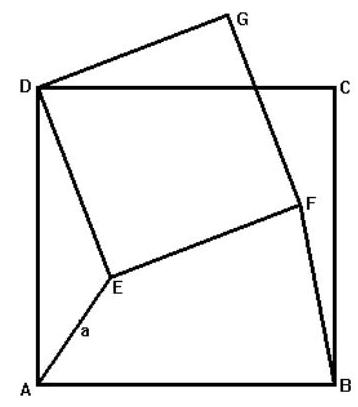
\includegraphics[max width=\textwidth, center]{2024_11_21_c97ae173c926e782bf17g-1}


\end{document}